\chapter{Objectives and Contributions}\label{chap:3-objetives}

This chapter presents the objectives of this thesis along with the open research problems it addresses (\hyperref[sec:Objectives]{Section} \ref{sec:Objectives}), together with the main contributions (\hyperref[sec:Objectives]{Section} \ref{sec:Contributions}), the thesis assumptions, main and secondary hypotheses, and restrictions (Sections \ref{sec:Assumptions}, \ref{sec:Hypotheses}, \ref{sec:Restrictions}), in addition to the evaluation plan for the stated hypotheses (within \hyperref[sec:Hypotheses]{Section} \ref{sec:Hypotheses}). It concludes with the research methodology and process followed during the development of this thesis (\hyperref[sec:ResearchMethodology]{Section} \ref{sec:ResearchMethodology}).


\section{Problem statement and objectives}\label{sec:Objectives}
\textit{Is it possible to use Explainable AI (XAI) techniques for explaining the results of applying unsupervised learning algorithms for anomaly detection within real-world contexts?} This is a step towards designing industry products that follow Responsible Artificial Intelligence (RAI) by design principles regarding XAI. As real-world industry contexts, two use cases within the telecommunications industry are considered. 
The first one is related to communications data (e.g. calls received in a Call Center, mobile data usage), where the aim is to identify and explain daily anomalies. This use case appears within the software product of LUCA\footnote{The brand \textit{LUCA} has undertaken several changes due to business needs. Nonetheless, we will keep mentioning it within the product names for compliance with legacy documentations and references, in order to enhance clarity.} Comms \parencite{LUCAComms}.
The second one is related to vehicle fuel consumption, where the aim is to identify vehicles with anomalous diesel and petrol fuel consumption, explaining the potential reasons behind it. This use case appears within the software product of LUCA Fleet \parencite{LUCAFleet}.

To address the main thesis question, the following research problems and objectives need to be considered:

\mybox{
    \begin{itemize}
    \item[\textbf{P1.}] On many situations, anomalies must be detected in an unsupervised manner, because there is no prior information about them. However, the output of anomaly detection models is reduced to a binary decision, not explaining the reasons behind it.
    \end{itemize}
}

To tackle this problem, the following objective is defined:
\begin{itemize}
\item[\textbf{O1.}] Considering the binary output of an unsupervised learning algorithm for anomaly detection, apply a model-agnostic post-hoc XAI technique that explains the relationship between the output and the input features in terms of rule-extraction or feature relevance explanations.
\end{itemize}

\mybox{
    \begin{itemize}
    \item[\textbf{P2.}] Even though XAI can be used for understanding the decision of a black box model, there is a lack of quantitative metrics for evaluating the quality of the explanations and benchmarking the techniques that have been used.
    \end{itemize}
}

The objectives pursued for this problem is:
\begin{itemize}
    \item[\textbf{O2.1}] Define metrics that measure the quality of the explanations by themselves, with respect to several XAI aspects.
    \item[\textbf{O2.2}] Analyse whether the results from the application of different XAI techniques differ significantly from each other, and propose novel alternatives that are best suited for specific contexts.
\end{itemize}

\mybox{
    \begin{itemize}
    \item[\textbf{P3.}] Explanations directly generated by existing XAI techniques may contradict domain knowledge, making them useless while also reducing the user's trust in the algorithm behind. It is important to ensure and evaluate that they are aligned with that prior knowledge.
    \end{itemize}
}

For approaching this problem, we consider the two use cases, LUCA Fleet and LUCA Comms, since there is prior domain knowledge that can be taken into account. For both cases, we define a first common objective, where the domain knowledge and user expectations should be considered within the explanation generation. Then, since the domain knowledge of factors affecting fuel consumption is well-researched, we define additional objectives regarding how to measure the explanation quality against that prior domain knowledge, and if the explanations are indeed aligned or not.
Thus, the objectives are:
\begin{itemize}
    \item[\textbf{O3.1}] Propose an algorithm that adjusts the explanation generation considering the prior domain knowledge and user expectations within the use cases covered.
    \item[\textbf{O3.2}] Propose an approach for measuring the quality of the explanations with respect to a priori beliefs.
    \item[\textbf{O3.3}] Conduct a study to analyse whether the explanations provided are aligned with the previous State of the Art (SOTA) regarding factors affecting fuel consumption.
\end{itemize}

\mybox{
    \begin{itemize}
    \item[\textbf{P4.}] XAI explanations should be tailored for the specific profile of the user that will receive them, taking into account both their expectations and domain knowledge. This is something identified within the XAI theory, but there is a lack of real-world research that shows how to properly approach it.
    \end{itemize}
}

This problem will be addressed only within the context of LUCA Fleet since, in this case, there are different user profiles that receive explanations: fleet managers and fleet operators.
\begin{itemize}
    \item[\textbf{O4}] Identify the different user profiles that will receive explanations, and adjust the content according to them.
\end{itemize}

%\begin{itemize}
%\item[\textbf{P5.}] Despite the fact that RAI by design can be used for AI-based products (regarding XAI), %there is a lack of research within the use case of anomaly detection in real-world industry contexts.
%\end{itemize}

%This final problem will also be addressed within the context of both use cases, LUCA Comms and  LUCA Fleet, through the following objective:

%\begin{itemize}
%\item[\textbf{O5.}] 
%\end{itemize}

\section{Contributions}\label{sec:Contributions}

The scientific contributions from this thesis aim to provide answers to the research problems mentioned in \hyperref[sec:Objectives]{Section} \ref{sec:Objectives}. They are divided into two layers: the first layer highlights the main conceptual contributions, while the second layer provides the technical contributions behind them. 

Regarding the \textbf{main contributions} (first layer):

\begin{itemize}
\item[\textbf{C1 }] \textbf{HyperRulEx} (\textbf{Hyper}cube \textbf{Rule} \textbf{Ex}traction). A framework that standardizes several rule extraction algorithms through the usage of hypercubes, which can be applied over anomaly detection algorithms. The framework includes several XAI metrics for analysing quantitatively the quality of the explanations. This is described in \hyperref[chap:4-rule-extraction]{Chapter} \ref{chap:4-rule-extraction}.

\item[\textbf{C2 }] An \textbf{empirical study of XAI} applied for explanation generation from unsupervised learning \textbf{anomaly detection} algorithms over \textbf{real-industry data} considering \textbf{prior domain knowledge}. It includes \textbf{adjusting the explanations} according to both that domain knowledge, as well as the \textbf{user profile} that receives them. It also involves defining \textbf{metrics} that take into account that prior knowledge for the explanation evaluation. 
This study covers two use cases: communications data and vehicle fuel consumption, which leads to the following contributions.

    \begin{itemize}
    \item[\textbf{C2.1 }] An approach for extracting rule-based explanations for \textbf{visually explaining} anomalies within the context of communications data, considering \textbf{prior domain knowledge} for generating the explanations. This is described in \hyperref[chap:5-comms-xai]{Chapter} \ref{chap:5-comms-xai}.
    
    \item[\textbf{C2.2 }] \textbf{RESYFEX} (\textbf{Re}commender \textbf{Sy}stem for Vehicle \textbf{F}uel Saving based on \textbf{Ex}plainable AI). A Recommender System (RecSys) built with XAI by design, that explains \textbf{fuel consumption anomalies} considering \textbf{a priori expert domain knowledge}, adjusts those explanations for \textbf{different user profiles}, and provide \textbf{actionable recommendations} for vehicle fuel saving.  This is described in \hyperref[chap:6-fleet-xai]{Chapter} \ref{chap:6-fleet-xai}.
    
    \end{itemize}
\end{itemize}

Regarding the \textbf{technical contributions, TC,} (second layer), we divide them in three sections, depending on the main contribution that is associated to them.

For \textbf{C1}, the technical contributions are related to the development of the rule-extraction framework, along with the metrics for the algorithm evaluation. In particular, they are:

\begin{itemize}
\item[\textbf{TC1 }] \textbf{SVM+Prototypes reloaded}, an algorithm for generating both post-hoc global and local counterfactual \textbf{rule-based explanations} that are model agnostic. This algorithm is a variant from a previous one within the literature, and comes with two alternatives methods.
\item[\textbf{TC2 }] \textbf{StabilityScore}, an algorithm for measuring the \textbf{stability} of the explanations provided by rule-extraction XAI techniques.
\item[\textbf{TC3 }] \textbf{DiversityScore}, an algorithm for measuring the \textbf{diversity} of the explanations provided by rule-extraction XAI techniques.
\item[\textbf{TC4 }] A \textbf{metric} for quantifying several aspects for measuring the quality of explanations from rule-based XAI techniques into a single metric.
\item[\textbf{TC5 }] An \textbf{open source library} for (C1), that includes the algorithms from (TC1), (TC2), (TC3), and (TC4). 
\end{itemize}

Regarding \textbf{C2.1}, the technical contributions focus on how to adjust the explanations generated in order to take into account prior domain knowledge within a use case with communications data. In particular:
\begin{itemize}
\item[\textbf{TC6 }] An algorithm for generating \textbf{visual explanations} in terms of counterfactual limits from a surrogate model that has a binary output. It explains that output with respect to one numerical continuous feature and any number of categorical ones. 
\item[\textbf{TC7 }] A \textbf{hyperparamer grid search method} for \textbf{One-Class Support Vector Machine (OCSVM)} based on MIES (\textit{measure the distance from samples to enclosing surfaces}. It complements (C4) in order to ensure that the counterfactual limits that separate outliers from inliers only have one upper and one lower limit, so they anomalous data points are always above or below the inliers, but not between them.

\end{itemize}

Finally, \textbf{C2.2}, the technical contributions are related to the usage of XAI techniques for providing fuel saving recommendations. Thus, they focus on the adjustments of XAI algorithms for generating those recommendations considering prior domain knowledge, as well as adjusting them for different user profiles. In particular:
\begin{itemize}
\item[\textbf{TC8}] \textbf{EBM\_var}, a variation over \textbf{EBM algorithm} that adjusts the feature-based explanations to account for possible differences between data subgroups that correspond to combinations of categorical feature values.
\item[\textbf{TC9}] An algorithm for ensuring that the feature-relevance local explanations provided by EBM, or by (TC8) algorithm, are \textbf{monotonic}. It includes a metric for measuring the \textit{monotonicity degree} of the results.
\item[\textbf{TC10}] An algorithm that turns the feature-relevance based local explanations from interpretable ML models, using EBM, os (TC7), or Constraint GA2M plus (CGA2M+) as references, into \textbf{actionable recommendations}.

\end{itemize}

Within the context of \textbf{C2.2}, the contributions also include empirical contributions (EC) in order to quantitatively evaluate the XAI explanations against that prior domain knowledge. In particular:
\begin{itemize}
\item[\textbf{C14}] A study over the XAI proposals from (C2.2) in order to see if their impact in the fuel usage is aligned with the factors affecting the fuel consumption that the literature describes.

\end{itemize}


\section{Hypotheses}\label{sec:Hypotheses}
The main hypothesis is that XAI can be used for explaining the results of applying unsupervised learning algorithms for anomaly detection within real-world contexts. This hypothesis is split into the following sub-hypotheses:

\begin{itemize}
\item[\textbf{H1.}] It is possible to apply post-hoc model-agnostic XAI techniques for explaining the anomalies detected by an unsupervised learning algorithm, and quantitatively measure the quality of the explanations with the usage of XAI-specific metrics.

\item[\textbf{H2.}] It is possible to take into account prior domain knowledge along with XAI for anomaly detection, either for adjusting the explanations generated or for benchmarking the quality of the explanations against it.

% TODO - Comentario: ¿valdría simplemente con decir que 'se ha incluido la propuesta' en esos productos para validar H3, o mejor dejar sólo H1 y H2.
%\item[\textbf{H3.}] It is possible to use XAI within real-world industry products, following a RAI approach, for both detecting and explaining the anomalies detected. 
\end{itemize}

% Poner aquí un comment de las evaluations
% Duda: Un unico capitulo para el evaluation de todas las contribuciones? Busco como poder condensarlo en uno?
The hypotheses defined previously are evaluated within \hyperref[sec:RuleExtractionEvaluation]{Section} \ref{sec:RuleExtractionEvaluation}, \hyperref[sec:ch5-evaluation]{Section} \ref{sec:ch5-evaluation} and \hyperref[sec:ch6-evaluation]{Section} \ref{sec:ch6-evaluation}. \hyperref[fig:EvaluationPlan]{Figure} \ref{fig:EvaluationPlan} shows a schema for the Evaluation Plan (including only the principal contributions, C1, C2 and C3).


%\section{Evaluation Plan}\label{sec:EvaluationPlan}
%The hypotheses defined in Section \ref{sec:Hypotheses} are described below (see Chapter XXX for all the details of the evaluation performed). Figure \ref{fig:EvaluationPlan} shows a schema for the Evaluation Plan (including only the principal contributions, C1, C2 and C3).

%\begin{itemize}
%\item[\textbf{E1.}] (for H1) The goal of this evaluation is to use XAI techniques (focusing on rule extraction and feature relevance) and apply them over unsupervised learning algorithms for anomaly detection, approaching them as a classifier with a binary output. The evaluation includes the usage of already existing and novel XAI metrics in order to benchmark the explanations provided. Thus, we can compare several techniques, and see if there are differences depending on the context, even though the techniques themselves are model agnostic.

%\item[\textbf{E2.}] (for H2) The goal of this evaluation is, to first elicit domain specific knowledge and user's expectations for the explanations, and use that information for adjusting the explanations generated by the XAI techniques considered, within the context of LUCA Comms and LUCA Fleet. For LUCA Fleet, the evaluation includes the usage of metrics related to the prior domain knowledge in order to see if the explanations regarding potential fuel saving are aligned. 

%\item[\textbf{E3.}] (for H3) The goal of this evaluation is to determine whether it is possible or not to develop a product following RAI principles (regarding XAI) that successfully detects and explains the anomalies detected by unsupervised models.
%\end{itemize}

\begin{sidewaysfigure}[h!]
  \centering
  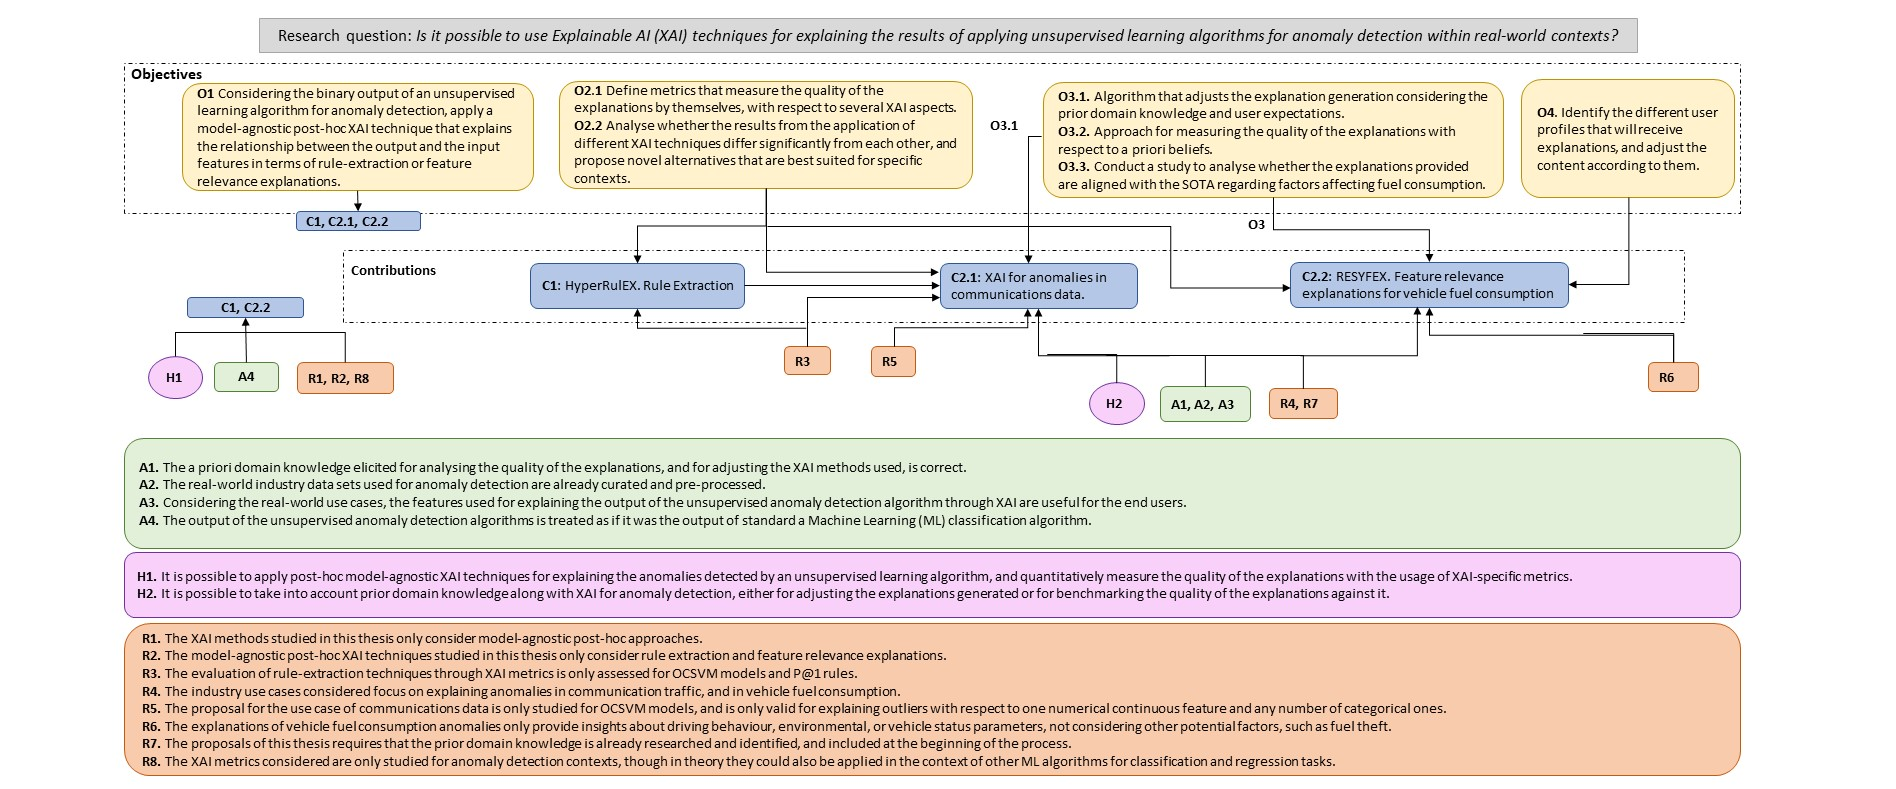
\includegraphics[width=0.85\columnwidth]{figures/EvaluationPlan.jpg}
  \caption{Relations between objectives, contributions, hypotheses, restrictions and assumptions of this thesis.}
  \label{fig:EvaluationPlan}
\end{sidewaysfigure}

\section{Assumptions}\label{sec:Assumptions}
This thesis was developed under a set of assumptions that help to explain the decisions taken for the achievement of the thesis goals; such assumptions are listed below:

\begin{itemize}
\item[\textbf{A1.}] The a priori domain knowledge elicited for analysing the quality of the explanations, and for adjusting the XAI methods used, is correct.

\item[\textbf{A2.}] The real-world industry data sets used for anomaly detection are already curated and pre-processed, eliminating noisy registers (e.g. sensor measurement errors). They also contain the most relevant features for explaining the potential outliers.  

\item[\textbf{A3.}] Considering the real-world use cases, the features used for explaining the output of the unsupervised anomaly detection algorithm through XAI are useful for the end users that are receiving them.

\item[\textbf{A4.}] The output of the unsupervised anomaly detection algorithms is treated as if it was the output of standard a Machine Learning (ML) classification algorithm.

% TODO - Comment: ¿Cómo que esta es 'strong'? ¿La quito, la dejo o la modifico?
%\item[\textbf{A4.}] The empirical metrics used for measuring the quality of the different types of explanations generated are assumed to be correct based on the previous literature.

\end{itemize}

\section{Restrictions}\label{sec:Restrictions}
The following restrictions define boundaries of the contributions of this thesis, highlighting future research problems than can be further pursued. These restrictions are:

\begin{itemize}
\item[\textbf{R1.}] The XAI methods studied in this thesis only consider model-agnostic post-hoc approaches.

\item[\textbf{R2.}] The model-agnostic post-hoc XAI techniques studied in this thesis only consider rule extraction and feature relevance explanations. Other alternatives, such as prototype-based explanations, are not researched.

\item[\textbf{R3.}] The evaluation of rule-extraction techniques through XAI metrics is only assessed for OCSVM models and P@1 rules.

\item[\textbf{R4.}] The industry use cases considered focus on explaining anomalies in communication traffic, and in vehicle fuel consumption. However, other use cases could be considered.

\item[\textbf{R5.}] The proposal for the use case of communications data is only studied for OCSVM models, and is only valid for explaining outliers with respect to one numerical continuous feature and any number of categorical ones.

\item[\textbf{R6.}] The explanations of vehicle fuel consumption anomalies only provide insights about driving behaviour, environmental, or vehicle status parameters, not considering other potential factors, such as fuel theft.

% No entiendo muy bien el comment the Oscar. Por que poner lo de 'independently of where it is taken from'? Lo que quiero decir aqui es que tiene que estar identificado e incluido desde el ppio.
\item[\textbf{R7.}] The proposals of this thesis requires that the prior domain knowledge is already researched and identified, and included at the beginning of the process.
%The domain knowledge considered for the use cases in this thesis is already well-researched within the previous literature, so the proposed solution includes it from the beginning, instead of gathering it from the end users. 

\item[\textbf{R8.}] The XAI metrics considered are only studied for anomaly detection contexts, though in theory they could also be applied in the context of other ML algorithms for classification and regression tasks.

\end{itemize}


\section{Research methodology}\label{sec:ResearchMethodology}
This section presents an overview of the research methodology followed during this thesis. To achieve the contributions related to the research problems described in \hyperref[sec:Objectives]{Section} \ref{sec:Objectives}, several methodology phases are defined, as indicated in \hyperref[fig:ResearchMethodologyFigure]{Figure} \ref{fig:ResearchMethodologyFigure}. Along with the phases, the figure depicts the activities carried out, and the contributions generated in each of those phases. The contributions are indicated though the appropriate bibliographic references.


\begin{itemize}

\item[1.] \textit{Domain Research Work.} An analysis of RAI is conducted, highlighting the importance of including XAI aspects during the design phase of AI-based products. As a result, we saw that this development approach was still an open area within real-world industry products. Because of that, we focused on applying it within two real-world industry products: LUCA Comms and LUCA Fleet.

\item[2.] \textit{Survey.} We conducted a review of the SOTA of both XAI and RAI, finding that even though there are many contributions for supervised ML models, there are areas where more research is needed. One of those areas is studying the applicability of XAI to unsupervised anomaly detection algorithms. We also saw a lack of research for XAI applied to anomaly detection within real-world industry use cases. Finally, we also discovered that the usage of quantitative metrics for assessing the quality of the explanations needed more research.

\item[3.] \textit{Development.} We first focused on studying rule extraction based techniques, since there was a lack of metrics regarding the measurement of the quality of the explanations. With this, we proposed a framework that standardizes the rule-extraction methods, and measures the quality of explanations with XAI metrics (C1). We then took the rule extraction approach for the use case of LUCA Comms, where the explanation generation needed to be adjusted in order to consider user's expectations and prior knowledge, leading to (C2.1). We also considered a third XAI approach by using feature relevance based techniques, and applying them within the context of vehicle fuel consumption (LUCA Fleet), leading to (C2.2), where the explanations generated must take into account prior domain knowledge. Within this last real-world use case, we also conducted an analysis in order to see if the final explanations are aligned with other aspects within the prior domain knowledge.

\item[4.] \textit{Implementation.} The three XAI approaches considered for explaining the output of anomaly detection algorithms lead to different final results and implementations. 
With (C1), an open source library was developed, providing a common framework for rule extraction, including XAI metrics for analysing the explanation quality. For (C2.1), the proposal is integrated within LUCA Comms product. Finally, for (C2.2), a fuel saving recommender system was developed, leading to a software prototype that is going to be included within LUCA Fleet in a future release.
\end{itemize}

\begin{figure}[h!]
\centering
  \begin{tabular}{c@{\qquad}c@{\qquad}c}
  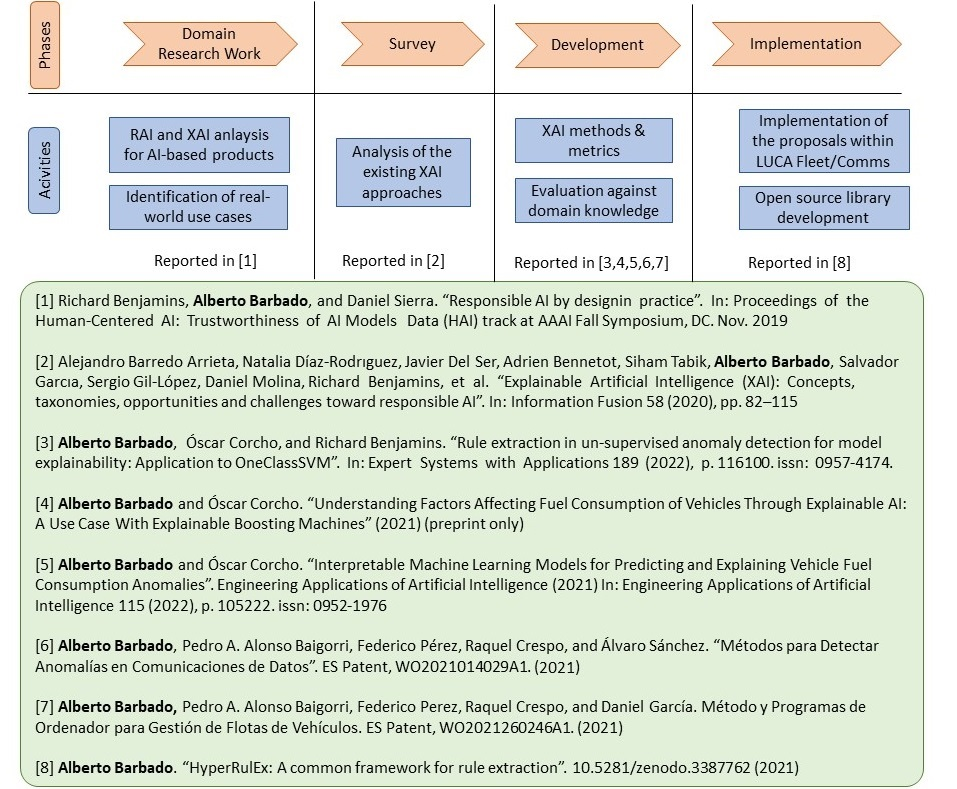
\includegraphics[width=0.9\columnwidth]{figures/ResearchMethodology.jpg}
  \end{tabular} 
  \caption{Phases of the thesis development, including the activities carried out during
each phase and the main publications derived from each phase.}
  \label{fig:ResearchMethodologyFigure}
\end{figure}


\newpage